\documentclass[12pt,oneside,letterpaper]{article}
\usepackage{longtable}
%\usepackage{fullpage}
\usepackage{hyperref} % Hyperlinks the table of contents automagically %
\usepackage{graphicx} % Embedding of images %
\usepackage{verbatim}
\usepackage{enumitem}

\newenvironment{packed_enumerate}{ %custom enumerate for single-spacing %
\vspace{-7mm}
\begin{enumerate}
  \setlength{\itemsep}{0pt}
  \setlength{\parskip}{0pt}
  \setlength{\parsep}{0pt}
}{\end{enumerate}
\vspace{-8mm}}

\pagestyle{headings}
\oddsidemargin 0.25in \textwidth 6.25in \topmargin 0.4in
\textheight 8.5in

\begin{document}

\title{\bfseries CALM: \\
Software Requirements Specification\\
version 2.0}

\author {
\large{Code a' la Mode}\\
\emph{Computer Science Department}\\
\emph{California Polytechnic State University}\\
\emph{San Luis Obispo, CA USA}\\
}

\date{October 25, 2012}
\maketitle \thispagestyle{empty}

\pagebreak
\tableofcontents

\addcontentsline{toc}{section}{Revision History}

\addcontentsline{toc}{section}{Credits}

\section*{Credits}
\begin{tabular}{|l|l|p{2.5in}|l|}
\hline
\textbf{Name}&\textbf{Date}&\textbf{Role}&\textbf{Version}\\
\hline
Neil Greene & October 10, 2012 & Author Section 6& 1.0\\
\hline
Halli Meth & October 10, 2012 & Co-Author Sections 1, 2, 7, A, B, C & 1.0\\
\hline
Daniel Crawford & October 10, 2012 & Co-Author Sections 1, 2, 7, A, B, C & 1.0\\
\hline
Alejandro Cervantes & October 10, 2012 & Author Section 4 & 1.0\\
\hline
Erik Sandberg & October 23, 2012 & Author Section 5 & 1.1\\
\hline
\end{tabular}

\section*{Revision History}
\begin{tabular}{|l|l|p{2.5in}|l|}
\hline
\textbf{Name}&\textbf{Date}&\textbf{Reason for Changes}&\textbf{Version}\\
\hline
Halli Meth&October 7, 2012&Initial version of UC-2&1.0\\
\hline
Daniel Crawford&October 7, 2012&Initial version of UC-4&1.0\\
\hline
Halli Meth&October 9, 2012&Add more detail to UC-2&1.0\\
\hline
\parbox[t]{1.25in}{Halli Meth \par Daniel Crawford\strut}&October 10, 2012&Initial version of Sections 1, 2, 7, A, B, C&1.0\\
\hline
Alejandro Cervantes&October 10, 2012&Added more detail to UC-1 and filled out Section 4&1.0\\
\hline
Erik Sandberg & October 10, 2012 & Initial version of UC-5 & 1.0\\
\hline
Erik Sandberg & October 13, 2012 & Initial version of Section 5 & 1.0\\
\hline
Daniel Crawford&October 18, 2012&Web Services Use Cases&1.1\\
\hline
Erik Sandberg & October 23, 2012 & Update Section 5 with Web Services & 1.1\\
\hline
\parbox[t]{1.25in}{Daniel Crawford \par Halli Meth\strut}&October 24, 2012&Added Web Services to Section 2&2.0\\
\hline
\parbox[t]{1.25in}{Daniel Crawford \par Halli Meth\strut}&October 24, 2012&Added Force.com Developer User Class to Section 2&2.0\\
\hline
\parbox[t]{1.25in}{Daniel Crawford \par Halli Meth\strut}&October 24, 2012&Added Web Services to Section 4&2.0\\
\hline
\parbox[t]{1.25in}{Daniel Crawford \par Halli Meth\strut}&October 24, 2012&Added detailed Functional Requirements (FR-6 - FR-30) to Section 4&2.0\\
\hline
Daniel Crawford & October 25, 2012 &Put requirements in Section 5 and 6 into tabular format&2.0\\
\hline
Daniel Crawford & October 25, 2012 &Removed redundant use cases from Section 3, edited some use cases based on feedback from Kevin Carr&2.0\\
\hline
Daniel Crawford & October 25, 2012 &Added Static User Data to glossary; removed old terms from glossary&2.0\\
\hline
\end{tabular}

\newpage

\section{Introduction}
\subsection{Purpose}
This SRS describes the software functional and nonfunctional requirements for release 1.0 of the CALM API and Dashboard. This document is intended to be used by the members of the project team that will implement and verify the correct functionality of the system. The document will also be used by our mentor, Kevin Carr, and direct supervisor, Dr. David Janzen.
\subsection{Document Conventions}
The following conventions are used in our document.\\
\begin{packed_enumerate}
\item Links appear in monospaced font.
\end{packed_enumerate}
\subsection{Intended Audience and Reading Suggestions}
\subsubsection{Developer}
Developers will primarily reference the functional and non-functional requirements in the SRS. These requirements will have a direct correlation to the features that they are implementing.\\
\textit{Suggested Sequence}\\
\begin{packed_enumerate}
\item Overall Description.
\item System Features.
\item Other Nonfunctional Requirements.
\item External Interface Requirements.
\end{packed_enumerate}
\subsubsection{Mentor (Kevin Carr)}
Our Mentor will use this document to ensure that our team is aware of 
all user needs for this project. Additionally, he shall ensure that 
the team is aware of Salesforce technologies and business rules.\\
\textit{Suggested Sequence}\\
\begin{packed_enumerate}
\item Overall Description.
\item Use cases.
\item System Features.
\item Other Nonfunctional Requirements.
\item External Interface Requirements.
\end{packed_enumerate}
\subsubsection{Supervisor (Dr. David Janzen)}
Our Supervisor will use this document to remain informed of our team's 
decisions and progress. \\
\textit{Suggested Sequence}\\
\begin{packed_enumerate}
\item Overall Description.
\item Use cases.
\item System Features.
\item External Interface Requirements.
\item Other Nonfunctional Requirements.
\end{packed_enumerate}
\subsection{Project Scope}
This project will provide a simple way for application developers, who 
are Salesforce customers, to track metrics about their product. 
Additionally, it will provide relevant graphs and reports for their 
product's marketers and business executives to utilize in making 
company decisions and tracking progress.
For more information please refer to our \textit{Vision and Scope Document}[1].
\subsection{References}
These resources may be useful alongside of this document.\\
\begin{packed_enumerate}
\item CALM Coders. \textit{CALM: Vision and Scope},\\ \url{http://users.csc.calpoly.edu/~hmeth/VisionAndScope.pdf}

\end{packed_enumerate}

\vspace{0.25in}
\section{Overall Description}
\subsection{Product Perspective}
The CALM API and Dashboard are a new system that replaces the tedious 
process of gathering and displaying user metrics of mobile 
applications. The context diagram in Figure D-1 illustrates the 
external entities and system interfaces for releases 1.0 and 2.0.
\subsection{Product Features}
\subsubsection{CALM API}
The CALM API will be integrated with the android mobile developer's 
application.\\
\textit{Features:}\\
\begin{packed_enumerate}
\item Record static user information (examples: Country, Locale, 
Platform Information, etc.).
\item Record any events that developer specifies (example: button 
click).
\item Record screen changes within a single instance of the 
application.
\item Upload recorded data to the mobile application team's Salesforce 
database.
\end{packed_enumerate}
\pagebreak
\subsubsection{CALM Dashboard}
The CALM Dashboard will allow the user to view a graphical 
representation of different data metrics recorded from the CALM API 
(above).\\
\textit{Features:}\\
\begin{packed_enumerate}
\item Display information about overall usage of the user's product 
application.
\item Display data summations from custom events.
\item Display information about screen flow within the user's product 
application.
\end{packed_enumerate}

\subsubsection{CALM Web Services}
The CALM Web Services will be provide a way to conveniently request metrics data from the Salesforce database.\\
\textit{Features:}\\
\begin{packed_enumerate}
\item Retrieve information about overall usage of the user's product application.
\item Retrieve data summations from custom events.
\item Retrieve information about screen flow within the user's product application
\end{packed_enumerate}

\vspace{0.25in}
The context diagram in Figure D-1 illustrates the data flow between 
our three systems and the Salesforce database.\\

\subsection{User Classes and Characteristics}
\begin{longtable}{|l|p{3.8in}|}
\hline
\textbf{User Class}&\textbf{Description}\\
\hline
Application Developer&Writes mobile applications who wishes to store 
data about their application usage. Some mobile application developers 
will wish to store custom data about their product. Application 
developers will only use the CALM API portion of our product.\\
\hline
Marketer&Uses graphs and statistical analysis to understand their 
product's user base. Different types of graphs will be applicable for 
marketers in different situations. For example, the graph needed to 
pitch a new marketing campaign will be different than the graph needed 
to show how effective past marketing campaigns have been. Marketers 
will only use the CALM Dashboard portion of our product.\\
\hline
Management&Use graphs to track user trends, customer retention, and 
other important business metrics. Managers will use this information 
in order to decide on further improvements for their product. Managers 
will only use the CALM Dashboard portion of our product.\\
\hline
Force.com Developer&Uses the CALM Web Services to retrieve metrics 
data. The Force.com Developer could be integrating this data into other 
custom reports for their organization. They could also be using the data 
to create their own custom dashboard that is more tailored to their needs.\\
\hline
\end{longtable}

\subsection{Operating Environment}
The CALM API will run on the Android-based mobile devices. This API 
will need to send data to Salesforce through REST or SOAP. The database will 
be validated and aggregated through APEX. The CALM Dashboard will run as a native Android application. 
It will receive data from the database through REST or SOAP, which includes the CALM Web Services.

\subsection{Design and Implementation Constraints}
\vspace{0.25in}
\begin{packed_enumerate}
\item Developer experience- No experience with Android SDK, REST, or 
Salesforce Database systems.
\item Salesforce API Usage constraint- limit on the number of REST API 
calls per day, per Salesforce user.
\item API must authenticate before sending data to Salesforce.
\end{packed_enumerate}

\subsection{User Documentation}
\vspace{0.25in}
\begin{packed_enumerate}
\item Open source code example of an implementation of the CALM API.
\item Quick API integration guide for Application Developers 
(webpage).
\end{packed_enumerate}

\subsection{Assumptions and Dependencies}
\textit{Assumptions}\\
\begin{packed_enumerate}
\item We will be using APEX for back end data aggregation.\\
\end{packed_enumerate}
\textit{Dependencies}\\
\begin{packed_enumerate}
\item We will be using Localytics as the foundation for our API.
\item We will use an existing tool to generate graphs.
\item We will be using OAuth to authenticate.
\end{packed_enumerate}

\subsection{Business Rules}
\begin{longtable}{|l|p{3.8in}|}
\hline
\textbf{Business Rule}&\textbf{Description}\\
\hline
BR-1 & Users must be authorized via OAuth to send or receive data from 
Salesforce.\\
\hline
BR-2 & Our product must not store personally identifiable information 
for more than 24 hours.\\
\hline
\end{longtable}

%%%%%%%%%%%%%%%%%%%%%%%%%%%%%%% USE CASES %%%%%%%%%%%%%%%%%%%%%%%%%%%%%%%
\section{Use Cases}

%%%%%%%%%%%%%%%%%%%%%%%%%%%%%%% Start UC-1 %%%%%%%%%%%%%%%%%%%%%%%%%%%%%%%
\subsection{\label{UC-1}Use Case 1: API - Recording Metrics}
\begin{longtable}{|r|p{3.8in}|}
\hline
Use Case ID:&UC-1\\
\hline
Use Case Name:&Logging An Event\\
\hline
Created by:&Alejandro Cervantes\\
\hline
Last Updated by:&Daniel Crawford\\
\hline
Date Created:&10-6-12\\
\hline
Date Last Updated:&10-25-12\\
\hline
Actors:&Application Developer\\
\hline
Description:&The app developer is programming an application that 
displays real-time statistics about the network usage for a given 
network. The developer's application will also gather metric data 
about how the application is used and then send the data to their 
Salesforce database to be stored for later use. The developer will be 
using the CALM API for logging and pushing metric data to the Salesforce
database.\\
\hline
Preconditions:&
\begin{packed_enumerate}
\item The app developer has already registered with Salesforce and 
owns a database in which they can store data.
\item The app developer has already configured the CALM API for use 
with their application.
\end{packed_enumerate}\\
\hline
Postconditions:&
\begin{packed_enumerate}
\item The logged event is successfully stored in their Salesforce 
database.
\end{packed_enumerate}\\
\hline
Normal Course:&\textbf{1.0 Stored logged event(s) in Salesforce 
database when application closes}\\
&
\begin{packed_enumerate}
\item Developer writes code, using the CALM API, that initializes the metric gathering session.
\item Developer writes code, using the CALM API, that logs an event whenever a user logs onto the network.
\item Developer writes code, using the CALM API, to send the data to the database when the app is closed.
\end{packed_enumerate}\\
\hline
Alternative Course:&\textbf{1.1 Store logged event(s) in Salesforce 
database whenever an event is logged (branch after step 2)}\\
&
\begin{packed_enumerate}
\item Developer writes code, using the CALM API, to send the data to 
the database right after the event is logged.
\end{packed_enumerate}\\
\hline
Exceptions:&\textbf{1.0E.1 Application unexpectedly exits before logs 
are sent. (at step 3)}\\
&
\begin{packed_enumerate}
\item The logs will be saved in a local database on the mobile device 
that the application is running on. 
\item The saved logs will be sent to the database when the application 
is opened the next time.
\end{packed_enumerate}\\
\hline
Includes:&None\\
\hline
Priority:&High\\
\hline
Frequency of use:&Once per individual application written.\\
\hline
Business Rules:&BR-1, BR-2\\
\hline
Special Requirements:&None\\
\hline
Assumptions:&None\\
\hline
Notes and Issues:&None\\
\hline
\end{longtable}
%%%%%%%%%%%%%%%%%%%%%%%%%%%%%%%%%%%% End UC-1 %%%%%%%%%%%%%%%%%%%%%%%%%%%%%%%%%%%% 

\subsection{\label{APILogScreen}Use Case 2: API - Log Screen}
App Developers can log a screen event when the application's screen changes.\\

\subsection{\label{APIClose}Use Case 3: API - Close Session}
App Developers can close the current recording session when the application 
closes.\\

%%%%%%%%%%%%%%%%%%%%%%%%%%%%%%%%%%%% Start UC-4 %%%%%%%%%%%%%%%%%%%%%%%%%%%%%%%%%%%% 
\subsection{\label{DashboardLogin}Use Case 4: Dashboard - Login}
\begin{longtable}{|r|p{3.8in}|}
\hline
Description:&Users can log in to the CALM Dashboard app with Salesforce 
login credentials.\\
\hline
Precondition:&
\begin{packed_enumerate}
\item User has installed the CALM Dashboard app.
\item User has opened the CALM Dashboard app.
\item User has valid credentials and permissions for their Salesforce 
account.
\end{packed_enumerate}\\
\hline
Postconditions:&
\begin{packed_enumerate}
\item User is logged into the CALM Dashboard app.
\end{packed_enumerate}\\
\hline
\end{longtable}
%%%%%%%%%%%%%%%%%%%%%%%%%%%%%%%%%%%% End UC-4 %%%%%%%%%%%%%%%%%%%%%%%%%%%%%%%%%%%% 

%%%%%%%%%%%%%%%%%%%%%%%%%%%%%%%%%%%% Start UC-5 %%%%%%%%%%%%%%%%%%%%%%%%%%%%%%%%%%%% 
\subsection{\label{DashboardSessionLength}Use Case 5: Dashboard - Average Session Length}
\begin{longtable}{|r|p{3.8in}|}
\hline
Use Case ID:&UC-5\\
\hline
Use Case Name:&Dashboard, Average Session Length Histogram\\
\hline
Created by:&Halli Meth\\
\hline
Last Updated by:&Daniel Crawford\\
\hline
Date Created:&10-7-12\\
\hline
Date Last Updated:&10-25-12\\
\hline
Actors:&Application Marketer\\
\hline
Description:&The application's marketer accesses the CALM Dashboard 
app from their android phone and chooses to view "Session Length." In 
response to the user's request, the system displays a histogram with 
requested data. The graph's goal is to show how much time users spent 
in a single session of the marketer's product (application). Each bar 
in the graph represents a group of users by session length. The height 
of the bar represents how many users there were in that time-slot. The 
bars are labeled by session length on the x-axis, and number of users 
on the y-axis. The marketer can also view the average and median 
session lengths in a simple table beneath the histogram.\\
\hline
Preconditions:&
\begin{packed_enumerate}
\item The company that the application marketer works for owns a 
database in which they can store data.
\item The application marketer has already registered with Salesforce 
and has access to the database from Precondition 1.
\item The application marketer has installed the CALM Dashboard app.
\item The application marketer has opened the CALM Dashboard app.
\item The application marketer has logged into their Salesforce 
account from Precondition 2 from the CALM Dashboard app.
\end{packed_enumerate}\\
\hline
Postconditions:&
\begin{packed_enumerate}
\item The application marketer has successfully viewed a graphical 
representation of their aggregated user data from the CALM Dashboard 
app.
\item The CALM Dashboard app closed without errors.
\end{packed_enumerate}\\
\hline
Normal Course:&\textbf{1.0 Use the CALM Dashboard app to view Session 
Length user data summations.}\\
&
\begin{packed_enumerate}
\item Marketer selects the Session Length graph option from CALM 
Dashboard app menu.
\item System displays the Session Length histogram.
\item Marketer views graphical representation of user's session 
lengths.
\item Marketer asks to exit.
\item System terminates use case.
\end{packed_enumerate}\\
\hline
Alternative Course:&none\\
\hline
Exceptions:&\textbf{1.0.E.1 No Session Length Data is available (at 
step 2).}\\
&
\begin{packed_enumerate} %%TODO(halli): Add options 2a, 2b, 3a, 3b
\item System displays an empty histogram with default labels. 
\item Application marketer chooses to return to home screen.
\item System terminates use case.
\item Marker starts Normal Course over. 
\end{packed_enumerate}\\
\hline
Includes:&UC-4 The user is able to log in to the CALM Dashboard 
application.\\
\hline
Priority:&High\\
\hline
Frequency of use:&Approximately one time per week by each marketer. 
Each marketer will use the Session Length histogram daily when new 
features are released in their product to view changes in usage.\\
\hline
Business Rules:&BR-1 Marketers may only view data in the CALM 
Dashboard app from Salesforce databases that they have access to. \\
\hline
Special Requirements:&None\\
\hline
Assumptions:&None\\
\hline
Notes and Issues:None&\\
&
\begin{packed_enumerate}
\item Default labels are: session length \{0-10s, 11-30s, 31-60s, 1- 3m, 3-10m, 10-30m, 30-60m, \textgreater1hr\}    number of users \ {1000, 2000, 3000, 4000, 5000+}
\end{packed_enumerate}\\
\hline
\end{longtable}
%%%%%%%%%%%%%%%%%%%%%%%%%%%%%%%%%%%% End UC-5 %%%%%%%%%%%%%%%%%%%%%%%%%%%%%%%%%%%% 

%%%%%%%%%%%%%%%%%%%%%%%%%%%%%%%%%%%% Start UC-6 %%%%%%%%%%%%%%%%%%%%%%%%%%%%%%%%%%%% 
\subsection{\label{DashboardEventFlow}Use Case 6: Dashboard - Viewing Events}
\begin{longtable}{|r|p{3.8in}|}
\hline
Use Case ID:&UC-6\\
\hline
Use Case Name:&Dashboard - View Event Flow\\
\hline
Created by:&Erik Sandberg\\
\hline
Last Updated by:&Daniel Crawford\\
\hline
Date Created:&10-10-12\\
\hline
Date Last Updated:&10-25-12\\
\hline
Actors:&Analyst\\
\hline
Description:&The Analyst accesses the Event Overview section of the CALM 
Dashboard App. A bar graph of frequency per event is shown. The Analyst taps on the bar for a particular event. A line graph that shows the frequency of that event over a period of time is displayed.\\
\hline
Preconditions:&
\begin{packed_enumerate}
\item User is logged in to the CALM Dashboard App.
\end{packed_enumerate}\\
\hline
Postconditions:&
\begin{packed_enumerate}
\item The Analyst has received new information about how people are 
using their application.
\end{packed_enumerate}\\
\hline
Normal Course:&\textbf{1.0 Use the CALM Dashboard App to view event details.}\\
&
\begin{packed_enumerate}
\item Analyst opens the Event Overview section of the CALM Dashboard App.
\item \label{displayEvents1}System displays a bar graph where each bar corresponds to an event, and the height of the bar corresponds to frequency.
\item \label{selectEvent}Analyst taps on a particular bar to view details about that event.
\item \label{displayEvents2}System displays a line graph showing the occurrence of the selected event over a period of time.
\item \label{displayEvents3}Analyst uses the back button on the device to go back to the Event Overview graph.
\item \label{repeat}Repeat steps \ref{selectEvent} and 
\ref{displayEvents3} until Analyst is done.
\item Analyst asks to see a different section.
\item System terminates use case.
\end{packed_enumerate}\\
\hline
Alternative Course:&None\\
\hline
Exceptions:&\textbf{1.0.E.1 No Event data is available (at step 
\ref{displayEvents1} or \ref{displayEvents2}}\\
&
\begin{packed_enumerate}
\item System displays message: ``No event data available''
\item Analyst asks to see a different section.
\item System terminates use case.
\end{packed_enumerate}\\
\hline
Includes:&Dashboard queries Database\\
\hline
Priority:&High\\
\hline
Frequency of use:&Several times per day for a couple days every couple 
weeks.\\
\hline
Business Rules:&BR-1\\
\hline
Special Requirements:&None\\
\hline
Assumptions:&None\\
\hline
Notes and Issues:&None\\
\hline
\end{longtable}
%%%%%%%%%%%%%%%%%%%%%%%%%%%%%%%%%%%% End UC-6 %%%%%%%%%%%%%%%%%%%%%%%%%%%%%%%%%%%% 

\subsection{\label{DashboardLineGraph}Use Case 7: Dashboard - Line 
Graph}
Users can choose to view a metric that is represented as 
a Line Graph.\\

\subsection{\label{DashboardBarChart}Use Case 8: Dashboard - Bar 
Chart}
Users can choose to view a metric that is represented as 
a Bar Chart.\\

\subsection{\label{WebService}Use Case 9: APEX Web Service - Get Events by App ID}
Force.com developers can access a collection of Events with a certain App ID.\\

\subsection{\label{WebService}Use Case 10: APEX Web Service - Get Events by Name}
Force.com developers can access a collection of Events with a certain App ID and specified name.\\

\subsection{\label{WebService}Use Case 11: APEX Web Service - Get Session by App ID}
Force.com developers can access a collection of Sessions with a certain App ID.\\

\subsection{\label{WebService}Use Case 12: APEX Web Service - Get Session by Date Range}
Force.com developers can access a collection of Sessions with a certain App ID within a specified date range.\\

%%%%%%%%%%%%%%%%%%%%%%%%%%%%%%%%%%%% End Use Case Section %%%%%%%%%%%%%%%%%%%%%%%%%%%%%%%%%%%% 

%%%%%%%%%%%%%%%%%%%%%%%%%%%%%%%%%%%%% System Features %%%%%%%%%%%%%%%%%%%%%%%%%%%%%%%%%%%%%%%%%%%%%%%%%%

\section{System Features}

%%%%%%%%%%%%%%%%%%%%%%%%%%%%%% System Feature 001 %%%%%%%%%%%%%%%%%%%%%%%%%%%%%%%%%%%%%%%
\subsection{Record and Upload Metrics} 
\subsubsection{Description and Priority}
The CALM API can be used to collect Static User Data, such as the user's country of origin, the 
platform of the user's device, approximation of their locale, etc. It 
can also be used to log specific events that the developer specifies, such as 
when a button is clicked, as well as track screen changes in the application. The API can also be used to send
the recorded data to a Salesforce database.\newline Priority = High.
\subsubsection{Stimulus/Response Sequences}

\begin{longtable}{|l|p{3.8in}|}
\hline
Stimulus:&Developer uses method call from the API to record Static User Data.\\
\hline
Response:&When used by the end-user, the mobile application shall record the Static User Data as specified by the developer.\\
\hline
Stimulus:&Developer uses method calls from the API to record custom events.\\
\hline
Response:&When used by the end-user, the application with the developer's code will collect and store the 
event data when it occurs during the application session.\\
\hline
Stimulus:&Developer uses the method call from the API that tells 
the application to send the data to the developer's database.\\
\hline
Response:&When used by the user, the application with the developer's code will send the logged data to 
the database at the time in the application's life cycle specified by 
the developer. This will typically be when the application cleanly exits.\\
\hline
\end{longtable}
 
\subsubsection{Functional Requirements}

\begin{longtable}{|l|p{3.8in}|}
\hline
\textbf{Requirement}&\textbf{Description}\\
\hline
FR-1&If the developer tells the system to log Static User Data. When used by the end-user, 
the application with the developer's code shall then collect Static User Data when 
a user starts up the application.\\
\hline
FR-2&If the developer tells the system to log specific events, such as 
a button click. When used by the end-user, the application with the developer's code shall then log the 
specified events when they occur as the user uses the application.\\
\hline
FR-3&If the developer tells the system to log an event whenever the 
application's screen is changed. When used by the end-user, the application with the developer's code shall then log an event whenever 
the application's screen changes.\\
\hline
FR-4&The system shall send any logged data to the developer's 
Salesforce database at the time in the application's life cycle 
specified by the developer.\\
\hline
\end{longtable}


%%%%%%%%%%%%%%%%%%%%%%%%%%%%%% System Feature 002 %%%%%%%%%%%%%%%%%%%%%%%%%%%%%%%%%%%%%%%
\subsection{Display Recorded Data}
\subsubsection{Description and Priority}
The CALM Dashboard can retrieve and display the logged metric data that was stored in 
the developer's Salesforce database.\newline Priority = High.
\subsubsection{Stimulus/Response Sequences}

\begin{longtable}{|l|p{3.8in}|}
\hline
Stimulus:&The user tells the system to display a graph of a certain 
variety of metric data.\\
\hline
Response:&The CALM Dashboard retrieves the necessary data. Then the data will be displayed in graphical form.\\
\hline
\end{longtable}
 
\subsubsection{Functional Requirements}

\begin{longtable}{|l|p{3.8in}|}
\hline
\textbf{Requirement}&\textbf{Description}\\
\hline
FR-5&The system shall prompt the user for their Salesforce login credentials when the Dashboard is started.\\
\hline
FR-6&The system shall attempt to obtain authentication to access the Salesforce database using the user's credentials. 
If authentication fails, the user shall be prompted for their credentials again (See FR-5).\\
\hline
FR-7&Once authenticated, the system shall let the user choose a type of graph to view.\\
\hline
FR-8&The system shall display a line graph showing number of sessions over a period of time.\\
\hline
FR-9&The system shall display a line graph showing number of users over a period of time.\\
\hline
FR-10&The system shall display a bar graph showing number of sessions during each hour of the day.\\
\hline
FR-11&The system shall display a bar graph showing number of users during each hour of the day.\\
\hline
FR-12&The system shall display a bar graph showing number of sessions for each device model.\\
\hline
FR-13&The system shall display a bar graph showing number of users for each device model.\\
\hline
FR-14&The system shall display a bar graph showing number of sessions for each network carrier.\\
\hline
FR-15&The system shall display a bar graph showing number of users for each network carrier.\\
\hline
FR-16&The system shall display a bar graph showing number of sessions for each country.\\
\hline
FR-17&The system shall display a bar graph showing number of users for each country.\\
\hline
FR-18&The system shall display a bar graph showing number of sessions for each device model.\\
\hline
FR-19&The system shall display a bar graph showing number of users for each device model.\\
\hline
FR-20&The system shall display a bar graph showing number of sessions for each Android OS version.\\
\hline
FR-21&The system shall display a bar graph showing number of users for each Android OS version.\\
\hline
FR-22&The system shall display a bar graph showing number of sessions for each app version.\\
\hline
FR-23&The system shall display a bar graph showing number of users for each app version.\\
\hline
FR-24&The system shall display a bar graph showing the number of each custom event. Each bar, corresponding to a custom event, shall be clickable by the user. (See FR-25)\\
\hline
FR-25&The system shall display a line graph showing number of occurrences for a given custom event over a period of time.\\
\hline
FR-26&The system shall display a tree-like graph showing the screen flow through the application.\\
\hline
FR-27&The system shall allow the user to create and view custom funnels.\\
\hline
FR-28&The system shall allow the user to specify a date range for any of the graphs listed in FR-8 through FR-27.\\
\hline
\end{longtable}

%%%%%%%%%%%%%%%%%%%%%%%%%%%%%% System Feature 003 %%%%%%%%%%%%%%%%%%%%%%%%%%%%%%%%%%%%%%%
\subsection{Web Services}
\subsubsection{Description and Priority}
The CALM Web Services provide an easy way for Force.com developers to access commonly requested metric data from the CALM database.
\newline Priority = High.
\subsubsection{Stimulus/Response Sequences}

\begin{longtable}{|l|p{3.8in}|}
\hline
Stimulus:&The user requests a certain type of data by invoking a Web Service.\\
\hline
Response:&The CALM Web Service retrieves the necessary data from the database and returns it to the user.\\
\hline
\end{longtable}
 
\subsubsection{Functional Requirements}

\begin{longtable}{|l|p{3.8in}|}
\hline
\textbf{Requirement}&\textbf{Description}\\
\hline
FR-29&The system shall return an APEX object representing a collection of events that correspond to the caller's request.\\
\hline
FR-30&The system shall return an APEX object representing a session that corresponds to the caller's request.\\
\hline
TBD&Convenience methods to gather event information.\\
\hline
\end{longtable}

%%%%%%%%%%%%%%%%%%%%%%%%%%%%%% END System Features %%%%%%%%%%%%%%%%%%%%%%%%%%%%%%%%%%%%%%%%


\section{External Interface Requirements}
\subsection{User Interfaces}

\begin{longtable}{|l|p{3.8in}|}
\hline
\textbf{UI Requirement}&\textbf{Description}\\
\hline
UI-1&The API shall contain methods to record the beginning and end of a session.\\
\hline
UI-2&The API shall contain a method to record an event.\\
\hline
UI-3&The API shall contain a method to record a screen view.\\
\hline
UI-4&The API shall contain a method to send recorded metrics to the Salesforce database.\\
\hline
UI-5&The Web Services shall provide methods to retrieve analytic information.\\
\hline
UI-6&The Dashboard shall be able to display histograms, bar graphs, and line graphs.\\
\hline
\end{longtable}

\subsection{Hardware Interfaces}

\begin{longtable}{|l|p{3.8in}|}
\hline
\textbf{HI Requirement}&\textbf{Description}\\
\hline
HI-1&The Dashboard shall run on Android devices.\\
\hline
HI-2&The Database shall be hosted on Salesforce.com servers.\\
\hline
HI-3&The Web Services shall be hosted on Salesforce.com servers.\\
\hline
HI-4&The API shall run on Android devices.\\
\hline
\end{longtable}

\subsection{Software Interfaces}

\begin{longtable}{|l|p{3.8in}|}
\hline
\textbf{SI Requirement}&\textbf{Description}\\
\hline
SI-1&The API shall transmit metrics data to the Database through a programmatic interface.\\
\hline
SI-2&The Database shall store metrics data that it receives from the API.\\
\hline
SI-3&The Dashboard shall request metrics data from the Database through a programmatic interface.\\
\hline
\end{longtable}

\subsection{Communications Interfaces}

\begin{longtable}{|l|p{3.8in}|}
\hline
\textbf{CI Requirement}&\textbf{Description}\\
\hline
CI-1&The API shall transmit the metrics data to the Database through the Internet with
either REST or SOAP protocol.\\
\hline
CI-2&The Dashboard shall transmit requests to the Database through the Internet
with either REST protocol or the Web Services.\\
\hline
CI-3&The Web Service shall transmit metrics data to the Dashboard through the Internet
with a SOAP protocol.\\
\hline
\end{longtable}

%%%%%%%%%%%%%%%%%%%%%%%%%%%%%% Non-Functional Requirements %%%%%%%%%%%%%%%%%%%%%%%%%%%%%%%%%%%%%%%%

\section{Other Nonfunctional Requirements}

\subsection{Performance Requirements}

\begin{longtable}{|l|p{3.8in}|}
\hline
\textbf{PE Requirement}&\textbf{Description}\\
\hline
PE-1&The Dashboard initial login screen shall load within 3 second of startup.\\
\hline
PE-2&The Dashboard shall load and display a graph within five seconds of attempting to view a graph.\\
\hline
PE-3&Downloading and installing the CALM package from the AppExchange should take no longer than 30 seconds. \\
\hline
PE-4&Downloading and installing the Dashboard application should take no longer than 2 minutes on the average 3G connection.\\
\hline
\end{longtable}

\subsection{Safety Requirements}

No Safety requirements have been identified.

\subsection{Security Requirements}

\begin{longtable}{|l|p{3.8in}|}
\hline
\textbf{SE Requirement}&\textbf{Description}\\
\hline
SE-1&The Dashboard shall require Salesforce.com log in credentials.\\
\hline
\end{longtable}

\subsection{Software Quality Attributes}

\begin{longtable}{|l|p{3.8in}|}
\hline
\textbf{SQ Attribute}&\textbf{Description}\\
\hline
SQ-1&A mobile application developer using the CALM API shall be able to integrate metric recording into their application in less than 10 minutes.\\
\hline
SQ-2&The CALM AppExchange Package shall be Salesforce.com certified.\\
\hline
SQ-3&A user of The Dashboard shall be able to navigate to any non-customized graph within 3 touches. \\
\hline
SQ-4&A user of The Dashboard shall be able to create any customized graph within 5 minutes.\\
\hline
\end{longtable}

%\section{Other Requirements}
%TBD

% I dont think we have other requirements?

\appendix
\section{Glossary}
\begin{longtable}{|l|p{3.8in}|}
\hline
\textbf{Term}&\textbf{Definition}\\
\hline
CALM API&The API a mobile application developer will use to gather and 
send data.\\
\hline
CALM Dashboard App&The end product application for Marketers and Managers.\\
\hline
CALM Database&The Salesforce database with the custom schema to store metrics data.\\
\hline
CALM Web Services&The public facing APEX Web Services for accessing data stored in the CALM Database.\\
\hline
Static User Data&Metrics about the user that are static for a given session. Includes the following: session ID, user ID, device model, country, network carrier, OS version, app version.\\
\hline
App ID&A unique ID that can be used by an Application Developer to identify a certain mobile application.\\
\hline
App Under Analysis&Android app that uses the CALM API.\\
\hline
\end{longtable}

\section{Analysis Models}
\subsection{Figure D-1: Context Diagram}
%insert diagram here
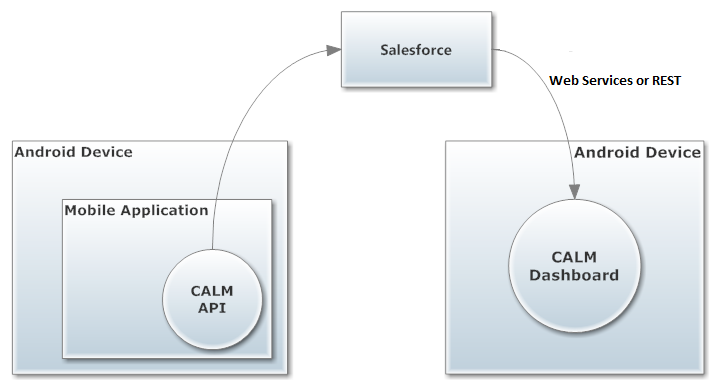
\includegraphics[scale=0.6]{context_diagram.png}

\section{Issues List}
\textit{Open Issues:}\\
\begin{packed_enumerate}
\item Team is unfamiliar with Salesforce technologies and 
terminologies.
\end{packed_enumerate}
\end{document}


